% !Mode:: "TeX:UTF-8"
\chapter{面向博物馆导览的对话式数字人展示设计实践}

\section{设计目标与整体架构}
\textbf{（1）设计概述}。如图\ref{fig-project-ui}所示，本研究面向博物馆学习场景，设计并实现了一个以数字人为核心交互媒介的对话式数字人导览原型系统。原型系统围绕观众在参观过程中的观看、提问、理解与跟随行为展开设计，将展品讲解、导览引导与互动交流组织在同一过程之中，使数字人能够陪伴观众完成从进入展厅、接触展品到持续理解和主动提问的完整导览体验。原型系统所关注的重点落在交互层面，即观众如何与数字人建立交流入口，如何在参观过程中持续进入讲解内容，以及如何在数字人的引导下形成更稳定的观看方向与理解节奏。

\begin{center}
    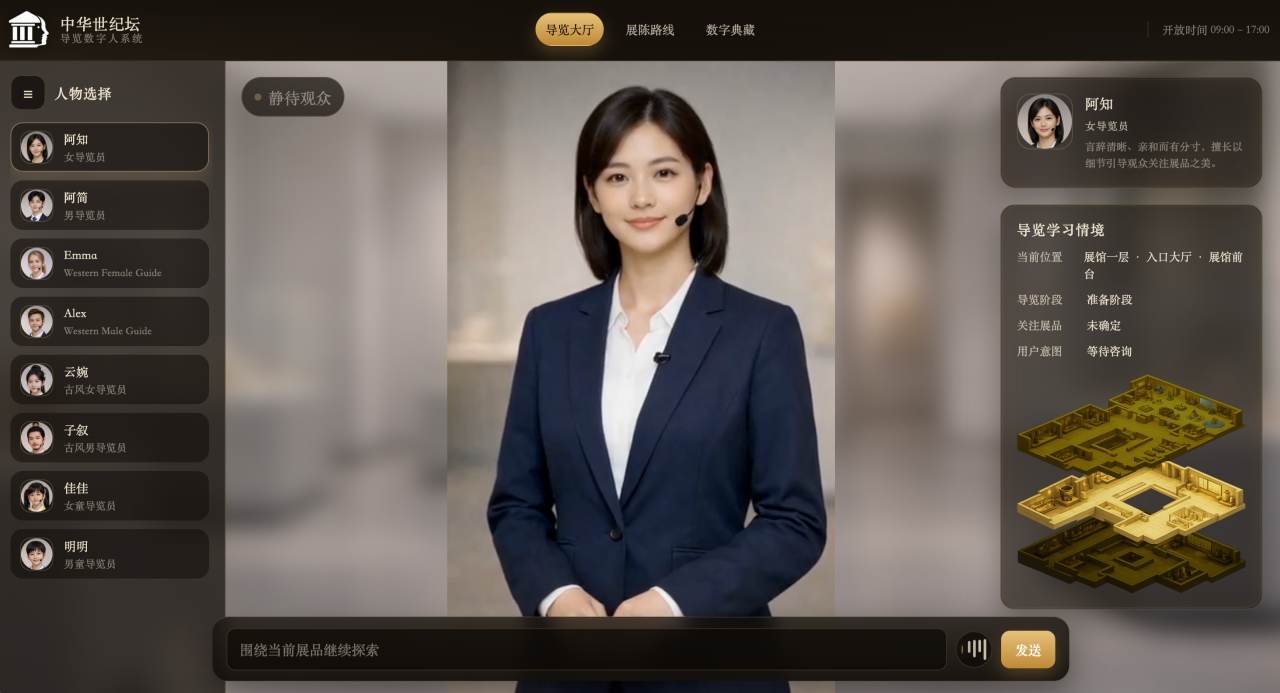
\includegraphics[width=\textwidth]{figure/figs/project-ui.png}
    \captionof{figure}{对话式数字人导览原型系统界面示意图}
    \label{fig-project-ui}
\end{center}

\textbf{（2）设计的交互构成}。围绕以上目标，本章的交互设计由三个相互衔接的部分构成。第一部分是对话组织设计，主要处理讲解内容如何被组织为可持续展开的互动过程，包括讲解单元的安排、导览路径的推进以及插问后的主线承接。第二部分是情境与状态设计，主要处理原型系统如何围绕参观位置、展品对象、会话进程和观众状态组织当前轮交互条件，并以此调节讲解进入点与展开深度。第三部分是具身导览交互设计，主要处理数字人如何通过动作、形象、声音和细粒度行为，将讲解重点、空间指向和交流关系转化为观众能够识别和跟随的外显线索。以下内容将围绕这三个部分展开具体说明。
系统与 CCEG 三维能力的映射关系如图\ref{fig-system-cceg-projection}所示。

\begin{center}
    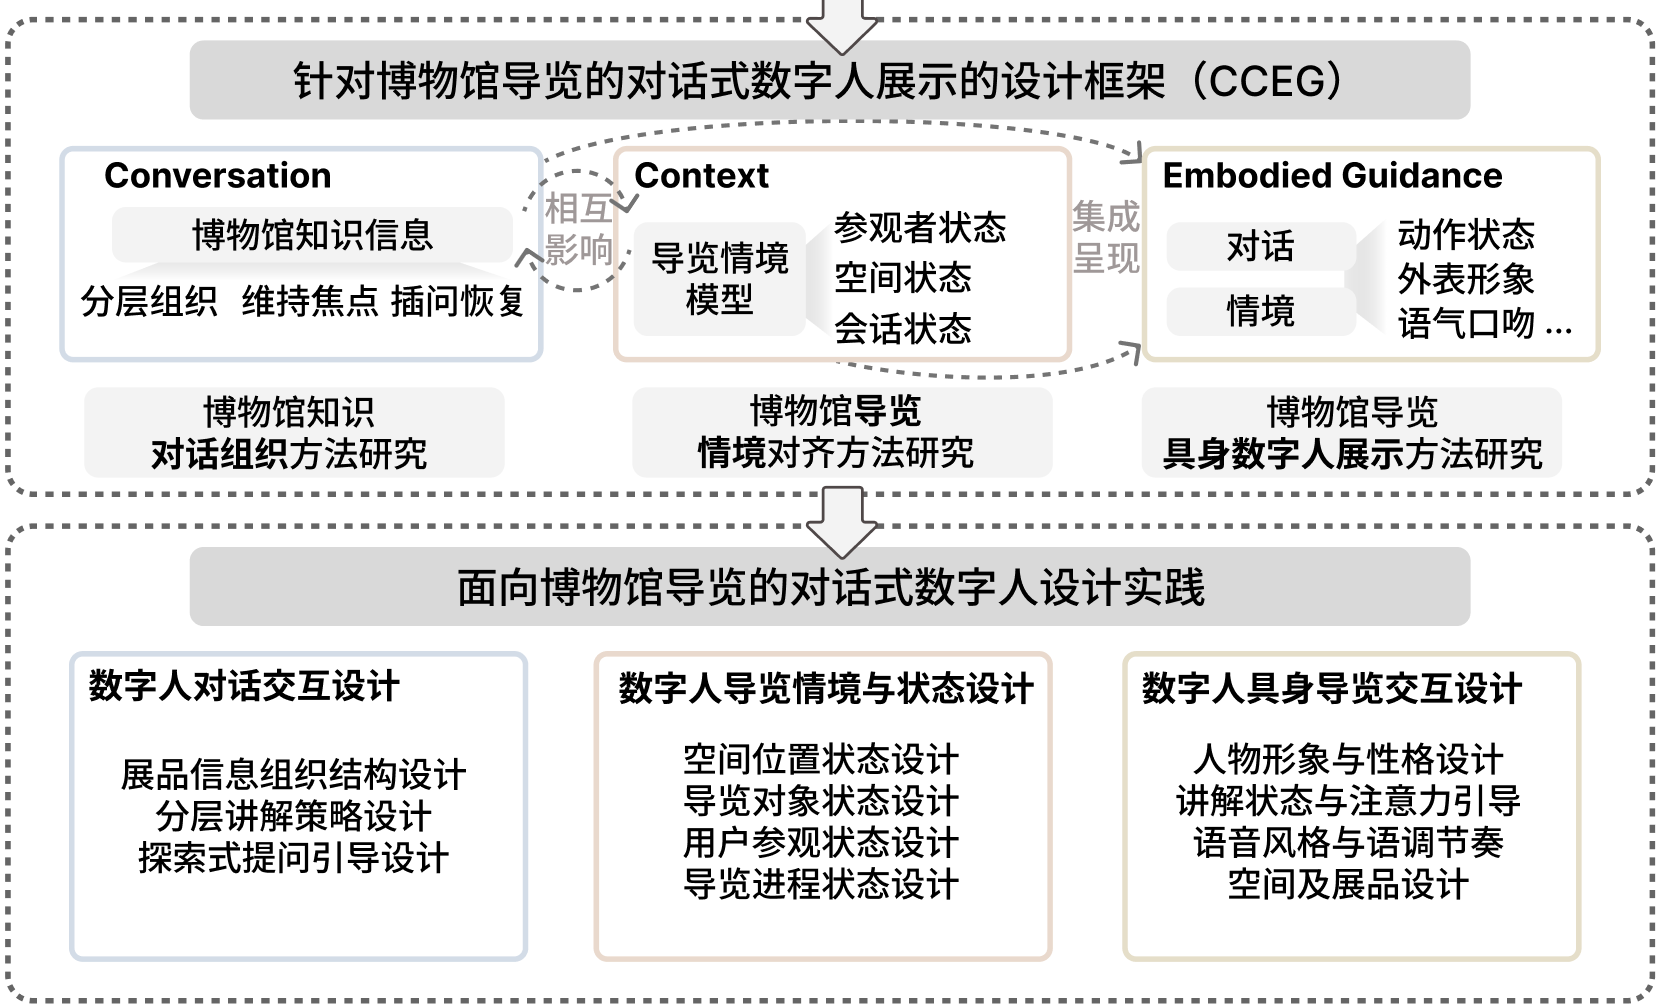
\includegraphics[width=\textwidth]{figure/figs/projection.png}
    \captionof{figure}{系统设计与 CCEG 三维能力映射关系示意图}
    \label{fig-system-cceg-projection}
\end{center}

\section{面向导览推进的对话组织设计}
\subsection{展品知识组织结构设计}
面向博物馆导览的对话组织，首先需要解决“讲解内容如何被组织”的问题。导览场景中的知识调用具有明显的过程性：系统需要在展厅整体介绍、展区进入、展品聚焦、细节展开与后续推荐等不同阶段之间切换，并根据当前参观位置与讲解目标选择合适的内容层次。基于这一需求，本研究将展品知识设计为一种面向导览调用的分层组织结构，使其能够服务于导览过程中的内容进入、层次展开与路径推进。如图\ref{fig-exhibit-knowledge-structure}所示，该结构以导览推进为主线组织展区与展品信息，并为后续讲解策略调用提供统一的数据基础。

\begin{center}
    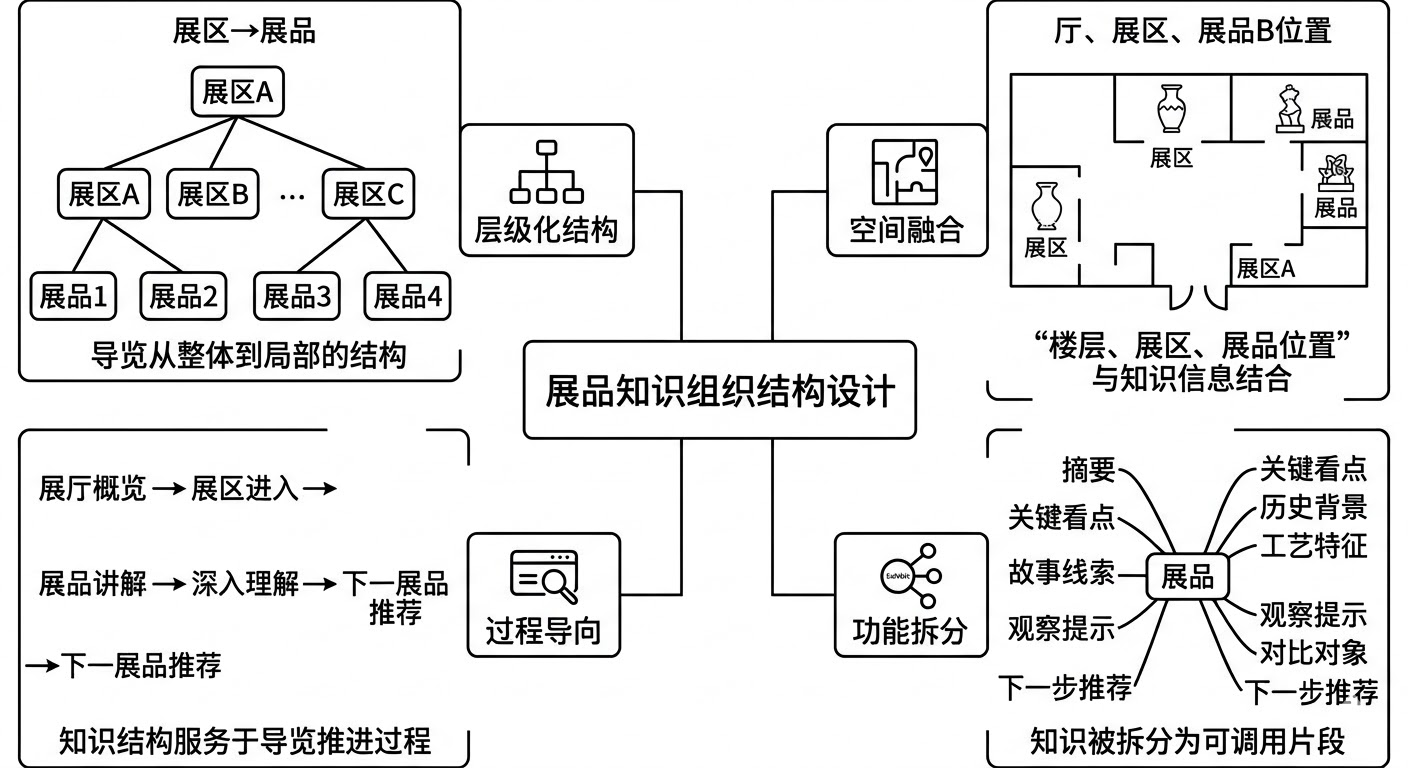
\includegraphics[width=\textwidth]{figure/figs/展品知识组织结构设计.png}
    \captionof{figure}{展品知识组织结构设计示意图}
    \label{fig-exhibit-knowledge-structure}
\end{center}

首先，在整体组织方式上，系统采用“展区-展品”两级知识结构，以展区作为导览中的上位单元，以展品作为具体讲解对象。展区层承担主题概览、空间定位与整体看点组织的功能，展品层承担对象说明、细节解释与延展内容调用的功能。这样的结构与博物馆导览中由整体到局部的讲解路径相一致，使系统能够在展厅整体介绍与具体展品讲解之间自然切换，并保持讲解对象的连续性与层次感。

其次，在知识内容的组织中，系统将空间信息与展品知识一并纳入同一结构之中。除展品本身的说明性内容外，知识条目同时维护展馆、楼层、展区位置描述以及展品所属展区等信息，使讲解内容能够与空间引导同步展开。这样一来，系统在组织导览时能够同时回答“讲什么”和“在哪里讲”两个问题，使展品知识与空间定位、路径引导形成统一的调用基础，从而更贴合真实参观情境中的导览需求。

再次，为适配不同讲解场景，系统对展品知识进行了功能化拆分，而非以单段描述文本进行存储。具体而言，展品层知识被划分为摘要、关键看点、历史背景、工艺特征、故事线索、观察提示、对比对象与下一步推荐等多个字段。这样的结构便于系统围绕不同导览目标选择内容：在概览阶段调用摘要与关键看点，在深入讲解阶段调用历史背景与工艺信息，在互动引导阶段调用观察提示与故事线索，在转场阶段调用下一步推荐。通过这种方式，知识组织从资料堆积转向导览任务驱动的结构设计。

最后，该知识结构直接服务于导览推进过程中的策略调用。系统需要依据当前导览阶段判断讲解进入点，依据用户关注决定讲解深度，依据展品关联关系生成后续推荐，依据不同受众模式调整表达内容。为此，知识结构在设计上围绕导览任务展开，使其能够支持展厅概览、展品聚焦、细节展开、儿童化表达与后续路径推荐等多种调用场景。由此，展品知识在系统中承担的角色不再只是信息存储，而是导览过程中的内容支撑与组织基础。

综上，本研究在展品知识组织上形成了四个设计特征：其一，采用“展区-展品”两级结构组织讲解内容；其二，将空间位置、展区归属与展品知识联合纳入同一结构；其三，将展品内容拆分为适配不同讲解任务的功能性字段；其四，使知识结构直接服务于导览阶段切换、讲解深度控制与后续路径推进。通过这样的设计，系统得以围绕博物馆导览的真实使用过程组织内容，并为后续的分层讲解、探索式提问与转场引导提供稳定支撑。

\subsection{分层讲解策略设计}
博物馆参观中的讲解通常呈现出由浅入深的理解过程。观众进入展厅时首先形成对展区主题的整体印象，随后在具体展品前建立对象识别，在停留与观察中逐步理解其历史背景与文化意义，最后通过比较与延展形成更完整的认识。基于这一参观特点，本系统将展品讲解组织为多个层次，使数字人能够根据导览阶段逐步展开讲解内容，从而形成由概览到深入的理解路径。如图\ref{fig-layered-explanation-strategy}所示，系统通过分层讲解机制将导览内容按阶段递进组织。

\begin{center}
    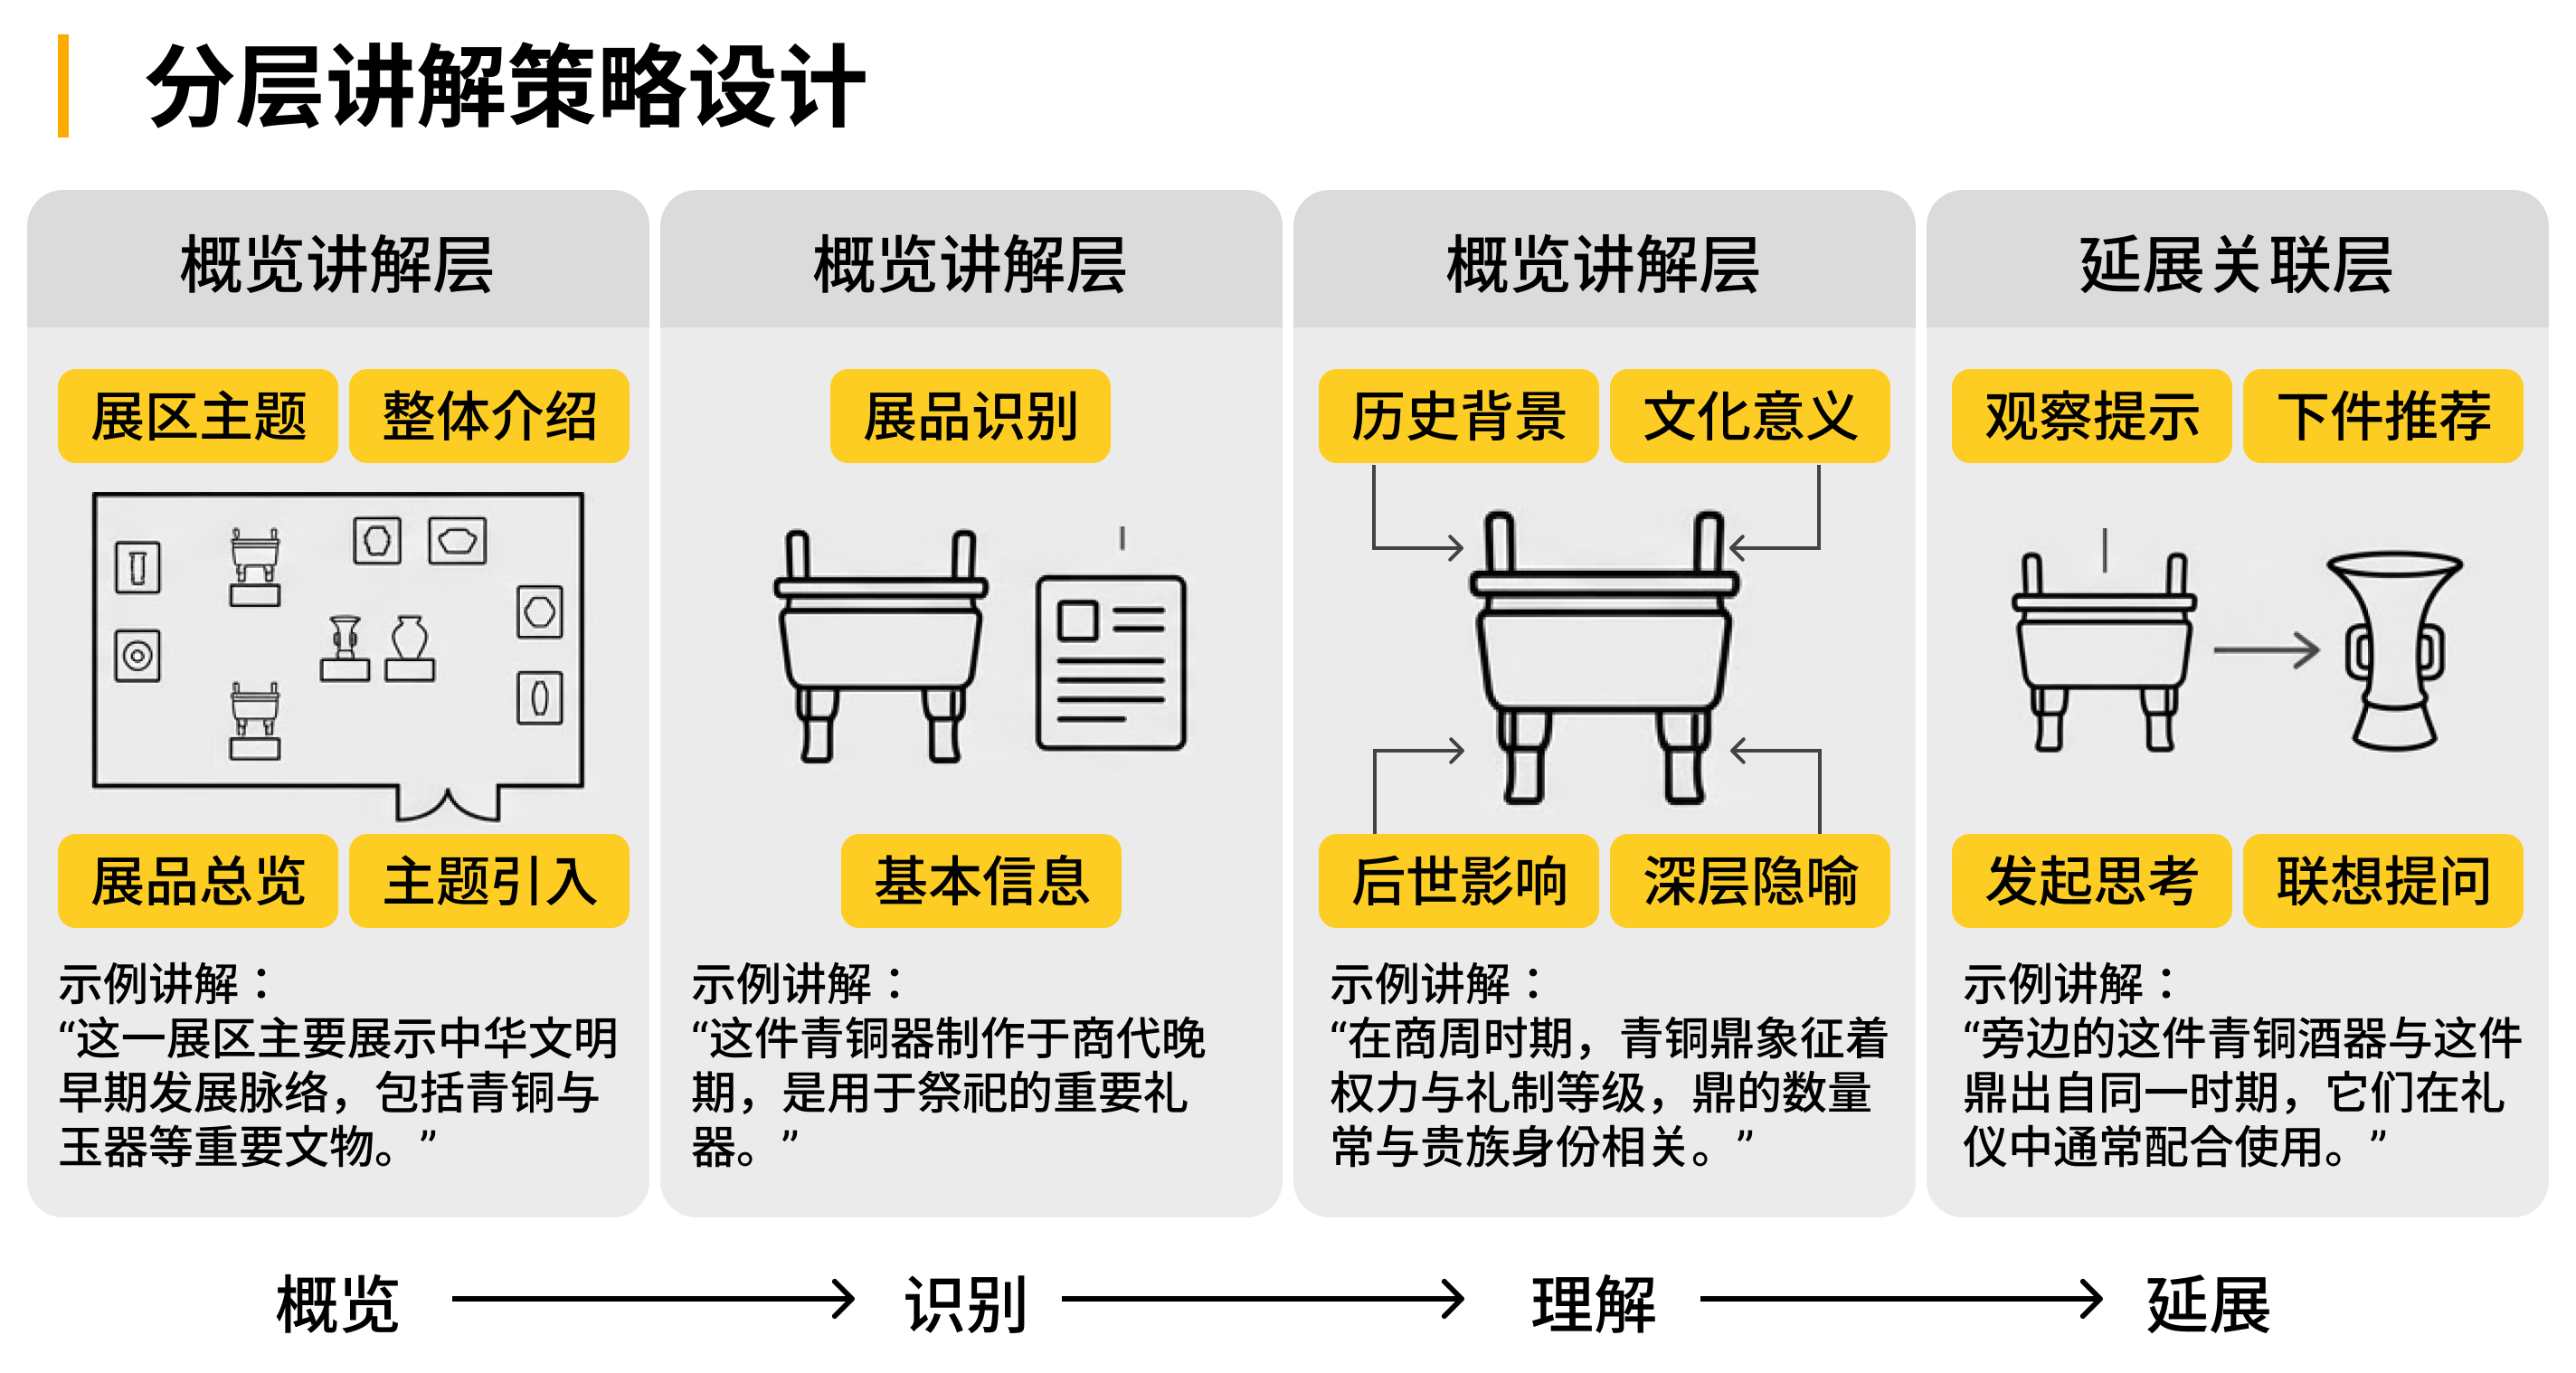
\includegraphics[width=\textwidth]{figure/figs/分层讲解策略设计.png}
    \captionof{figure}{分层讲解策略设计示意图}
    \label{fig-layered-explanation-strategy}
\end{center}

\textbf{（1）概览层讲解}。在导览开始阶段，系统首先提供概览层讲解。这一层的内容用于建立参观入口，帮助观众快速理解当前展区的主题与整体内容。例如，当观众进入“文明源流”展区时，数字人可以先进行整体介绍，如：“这一展区主要展示中华文明早期的发展脉络，其中包括青铜礼器、玉器以及早期文字等重要文物。”这种讲解重点在于建立背景与主题，使观众对展区形成整体印象。

\textbf{（2）基础层讲解}。当观众将注意力集中到具体展品时，系统进入基础讲解层。这一层的内容围绕展品本身展开，帮助观众识别对象并理解其基本信息。例如，当观众停留在一件青铜鼎前，系统可以介绍：“这件青铜鼎制作于商代晚期，是当时用于祭祀的重要礼器。鼎身铸有典型的饕餮纹，体现了当时青铜铸造技术的成熟。”这一阶段的讲解重点在于回答观众最直接的问题，即“这件展品是什么”。

\textbf{（3）深入层讲解}。随着观众继续停留或提出进一步问题，系统可以进入深入讲解层。这一层用于解释展品背后的历史背景、文化意义或工艺特征，使观众从识别对象进入理解阶段。例如，在继续讲解青铜鼎时，系统可以进一步说明：“在商周时期，青铜鼎不仅是一种器物，也象征着权力与礼制等级。鼎的数量与大小常常与贵族身份相关。”通过这样的内容展开，观众能够理解展品在历史文化中的地位。

\textbf{（4）延展层讲解}。当当前展品讲解接近结束时，系统会通过延展层讲解引导观众继续探索。例如，数字人可以提出观察提示或推荐下一件展品：“如果您仔细观察鼎身的纹饰，可以看到饕餮纹两侧还有细小的云纹装饰。旁边这件青铜觚与这件鼎出自同一时期，它们在礼仪中通常配合使用。”这样的讲解能够帮助观众将注意力从单件展品扩展到相关对象，并自然进入下一段导览。

通过这种多层次讲解方式，系统能够在不同导览阶段选择合适的内容深度。观众在导览过程中先建立整体印象，再识别具体对象，随后理解其历史意义，并在比较与延展中形成更完整的知识结构。讲解内容随着参观过程逐步展开，使数字人导览更符合真实参观中的理解节奏，也为后续的提问互动与导览转场提供了清晰的组织基础。

\subsection{探索式提问引导设计}
在博物馆导览场景中，提问是连接讲解内容与观众行动的重要手段。观众在参观过程中往往处于持续移动与观察的状态，很少持续主动发问，因此系统需要通过适当提问将观众从单纯听讲逐步引导到观察、选择和继续探索的参与状态。本系统在对话设计中将提问作为导览推进的重要机制，通过不同类型的问题维持参观节奏，并为观众提供新的探索入口。

\textbf{（1）阶段化提问引导机制}。系统根据导览进程动态调整提问方式，使提问能够与当前导览任务保持一致。在引路阶段，提问主要用于确认路径与行动，例如“要不要我带您先去看看这个展厅的代表展品？”；在展厅介绍阶段，提问用于帮助观众确定兴趣方向，例如“这个展厅里您想先看礼器还是玉器？”；在展品介绍阶段，提问用于推动理解深化，例如“您想继续听工艺细节，还是了解它背后的历史背景？”；在展品聚焦阶段，提问可以引导观察，例如“您可以注意一下它表面的纹饰，您觉得哪一部分最特别？”；在讲解接近收束时，提问则用于引导后续参观路径，例如“您想继续看这一时期的其他器物，还是转到下一个展区？”通过这种方式，提问与导览阶段形成对应关系，使对话能够随着参观过程逐步展开。

\textbf{（2）围绕对象、观察与路径的提问组织}。从参观任务角度看，博物馆导览中的探索主要集中在三个方面：选择观看对象、确定观察方式以及决定后续路径。因此，本系统将探索式提问围绕这三个维度进行组织。一类问题用于引导对象选择，例如“您想先看这一展区的代表展品，还是先整体了解展区主题？”；一类问题用于引导观察方式，例如“您注意到这件器物腹部和耳部的纹饰有什么不同吗？”或“这件器物和旁边那件相比，您觉得哪一件更强调礼仪功能？”；另一类问题用于推动参观路径，例如“您想继续看看同一时期的器物，还是去下一个展区？”这种组织方式使提问能够在内容理解与参观推进之间建立联系，使观众在不同层面的探索之间自然转换。

\textbf{（3）面向低负担交互的简短回应承接}。现场参观中的交流通常具有简短、碎片化的特点。观众在展厅里很少给出完整指令，更常见的是“好”“继续”“下一件”“那边呢”这样的简单回应。因此，本系统在提问设计中预留了简短回应的承接方式，使观众能够通过低成本表达完成确认与切换。例如，当系统提问“您想继续听细节，还是看下一件？”时，观众只需回答“细节”或“下一件”；当系统提问“要不要先去代表展品那里看看？”时，回应“好”即可继续导览；当系统提问“您想继续停留，还是转到下一个展区？”时，回答“走吧”也可以被系统自然接续。这种设计使交互方式更贴近真实参观情境，使观众能够在不打断参观节奏的情况下持续参与对话。

\section{面向现场导览的情境状态设计}
\subsection{空间位置状态设计}
博物馆现场导览具有鲜明的空间性特征。观众的参观活动总是发生在具体展馆、楼层、展区与展品分布之中，导览过程也随着空间移动不断推进。数字人若缺少对当前位置与空间关系的持续维护，讲解内容就容易与现场脱节，难以完成从入口引导、展区切换到对象聚焦的连续组织。因此，本系统首先围绕现场参观中的空间条件设计空间位置状态，使数字人能够在导览过程中明确“当前在哪里”“接下来去哪里”以及“当前位置适合讲什么”。

\textbf{（1）空间位置状态的分层表示}。在状态表示上，系统对空间位置进行了分层维护，主要包括当前展馆、当前楼层、当前区位、当前展区以及当前是否处于移动或引路中的状态。展馆与楼层状态用于确定参观活动所处的整体空间层级，支持在较大范围内组织导览路径；区位状态进一步描述观众所在的具体区域，如入口大厅、前台服务区或某一展区内部位置；展区状态则用于将当前位置与具体讲解单元相连接，使系统能够把空间位置与展厅主题、展品分布和导览任务对应起来。同时，系统还维护当前是否处于移动、引路或停留中的状态，以区分“正在前往下一地点”和“正在当前地点展开讲解”这两类不同导览情形。

\textbf{（2）空间位置状态服务导览路径组织}。空间位置状态首先服务于导览路径组织。在导览开始阶段，系统需要根据当前位置确定合适的进入点，例如当观众位于入口大厅时，数字人会优先进行展厅整体介绍，并提供“先从文明源流展区开始”这样的引导建议；当观众已经位于某个展区入口时，系统则可以直接进入展区概览阶段，而不再重复入口说明。在引路场景中，空间位置状态还用于支持“从哪里到哪里”的路径推进，例如从入口大厅进入文明源流展区，或从当前展厅切换到下一展厅。通过这种状态维护，导览过程能够围绕真实空间路径持续展开，而不是停留在脱离场景的知识问答中。

\textbf{（3）空间位置状态影响讲解内容进入方式}。空间位置状态还影响讲解内容的进入方式。同一类知识在不同空间位置下具有不同的组织方式：当观众位于展区外部时，系统更适合提供主题概览与方向提示；当观众已进入展区并停留在具体区域时，系统更适合围绕当前展区的代表内容展开讲解；当观众已经靠近某件展品时，系统则可以进一步进入对象识别与细节说明。例如，在入口大厅中，数字人可以说“这一层主要分为文明源流、书画文人、世界经典和互动体验几个展区”；当位置状态更新为“文明源流展区”后，讲解会切换为该展区的主题介绍；当位置进一步落到某件青铜礼器附近时，系统才进入该展品的具体说明。由此，空间位置状态成为讲解进入点选择的重要依据。

\textbf{（4）空间位置状态支持可视化与具身表达联动}。此外，空间位置状态也为后续情境可视化与具身表达联动提供基础。前端界面中的“当前位置”显示，正是对该状态的可视化呈现，它使用户能够清楚理解当前导览所处的位置与阶段；在具身表达层面，引路阶段、停留阶段和展品讲解阶段也会对应不同的动作与表达方式。例如，当系统判断当前处于引路状态时，数字人更适合采用指向或邀请式动作；当系统判断当前位置已经切换到目标展区后，数字人则进入相对稳定的讲解状态。空间位置状态因此不只是路径管理变量，也构成了导览内容组织与数字人行为切换的重要前提。

综上，空间位置状态设计是现场导览情境维护的基础层。通过对展馆、楼层、区位、展区与移动状态的联合维护，系统能够在导览过程中持续把握观众所处的空间位置，并据此组织路径引导、讲解进入与展厅切换。这一状态设计使数字人能够围绕真实参观场景展开导览，从而为后续的导览对象识别、进程维护与交互推进提供稳定支撑。

\subsection{导览对象状态设计}
在博物馆导览过程中，空间位置能够回答“观众现在在哪里”，而导览对象状态则进一步回答“系统当前围绕什么进行讲解”。对于数字人导览而言，仅知道观众位于某个展区并不足以组织有效讲解，系统还需要明确当前聚焦的是哪一展区、哪一件展品，以及该对象已经讲到什么程度。只有这样，数字人才能在展区概览、对象识别、细节解释与后续推荐之间形成连续的讲解过程。因此，本系统在空间位置状态之外进一步设计导览对象状态，用于持续维护当前讲解对象及其相关组织关系。

\textbf{（1）导览对象状态的表示结构}。在状态表示上，系统主要维护当前聚焦展区、当前聚焦展品、当前讲解层次以及当前展区内尚未讲解对象等信息。当前聚焦展区用于说明系统当前围绕哪个展厅单元展开导览，例如“文明源流展区”或“书画文人展区”；当前聚焦展品用于标识系统正在讲解或准备讲解的具体对象，例如某件青铜鼎、玉器或书画作品；当前讲解层次用于区分该对象当前处于简要介绍、基础讲解还是深入讲解阶段；尚未讲解对象状态则用于记录当前展区内仍可继续导览的展品，为后续的延展推荐和转场组织提供依据。这些状态共同构成系统对“当前讲解对象”的持续维护，使导览内容能够在对象层面保持稳定和连续。

\textbf{（2）导览对象状态服务对象确定与切换}。导览对象状态首先服务于讲解对象的确定与切换。当观众刚进入某一展区时，系统的聚焦对象通常仍停留在展区层，数字人会先介绍展区主题与代表内容；当观众进一步靠近某件展品或通过交互表达出明确兴趣时，系统会将聚焦对象从展区切换到展品层。例如，数字人在文明源流展区中可以先说“这一部分主要展示中华文明早期的重要礼器与器物”；当观众停留在青铜礼器区域后，系统便将当前聚焦展品更新为某件青铜鼎，并进入对象讲解阶段。通过这样的对象切换，导览能够从整体展区介绍自然过渡到具体展品说明。

\textbf{（3）导览对象状态支持讲解深度调节}。导览对象状态还影响讲解深度的调节。同一件展品在导览中往往要经历由浅入深的展开过程，因此系统需要判断当前对象是处于初步识别阶段，还是已经进入深入解释阶段。例如，当某件展品第一次进入讲解时，数字人可以先说明其名称、年代和基本用途；当观众继续停留或选择深入了解时，系统会把当前讲解层次更新为更深入的状态，并补充该展品的历史背景、文化意义或工艺特点。以青铜鼎为例，初次讲解时系统可以介绍“这是一件商代晚期的青铜礼器”；当导览继续推进时，则可以转入“它在当时礼制中的象征意义”或“鼎身纹饰的工艺特点”。这样，导览对象状态就不仅标识“讲的是哪一件”，也标识“讲到了哪一层”。

\textbf{（4）导览对象状态支撑展区内部内容延展}。此外，导览对象状态为展区内部的内容延展提供依据。博物馆导览很少在一件展品讲解完成后直接终止，更多时候需要继续在同一展区内推荐相关对象，或提示观众转向下一类展品。因此，系统还需要知道当前展区内有哪些对象已经讲过、哪些对象仍未展开。例如，在完成青铜鼎的介绍后，系统可以根据未讲对象状态推荐“旁边这件青铜觚与刚才这件鼎属于同一时期，可以一起帮助理解礼器组合的使用方式”；如果当前展区中的代表展品已经基本覆盖，系统则可以进一步组织转入下一展区的导览。由此，导览对象状态成为展区内部讲解推进和对象衔接的重要依据。

\textbf{（5）导览对象状态的前端可视化表达}。前端界面中的“当前关注展品”正是导览对象状态的可视化表达。它使用户能够清楚感知当前导览所围绕的核心对象，也让系统的讲解过程具有更强的可解释性。当该字段显示为“未确定”时，观众能够理解当前仍处于展区概览或路径引导阶段；当该字段更新为具体展品名称时，说明导览已经进入对象聚焦阶段。这样的可视化设计使对象状态不只存在于后台逻辑中，也成为用户理解当前导览进程的一部分。

综上，导览对象状态设计承担着讲解对象识别、对象切换、讲解深度控制与对象延展推荐等多重作用。通过对当前聚焦展区、当前聚焦展品、当前讲解层次以及未讲对象集合的持续维护，系统能够围绕“当前在讲谁”建立稳定的内容组织基础，使数字人导览在展区概览与展品聚焦之间形成自然衔接，并为后续的导览进程维护与交互推进提供明确对象依据。

\subsection{用户参观状态设计}
在现场博物馆导览中，用户的参观状态会随着空间移动、对象停留与互动反馈持续变化。观众进入展厅初期通常更需要整体介绍与方向提示；在停留于具体展品前时，会逐步转向对象识别与细节观察；当兴趣进一步聚焦时，则更适合进入背景解释与延展理解阶段；而在当前对象讲解接近结束时，观众又会进入是否继续停留或转向下一对象的选择状态。数字人若缺少对这些参观状态的识别与维护，导览内容就容易出现节奏失配，例如在观众尚未建立对象识别时过早进入深入解释，或在观众已经产生持续兴趣时仍停留在简略介绍层。因此，本系统在情境状态设计中加入用户参观状态，用于描述观众此刻处于何种参观阶段，并为讲解深度调节和导览策略切换提供依据。

\textbf{（1）用户参观状态的表示结构}。在状态表示上，系统将用户参观状态概括为初始进入、跟随浏览、停留观察、聚焦理解、深入探索和转场准备六类。初始进入状态通常出现在导览开始或刚进入新展区时，此时用户尚未形成明确关注对象，更需要整体背景和方向提示；跟随浏览状态表示用户正在跟随数字人的导览路径进行移动或整体观看，此时讲解应保持简洁并突出展区主题；停留观察状态表示用户已经在某一展品或区域前短暂停留，系统可以开始围绕该对象提供基础说明；聚焦理解状态表示用户的注意力已经稳定指向某件展品，适合进入对象识别与关键特征讲解；深入探索状态表示用户通过停留、提问或继续选择表现出明确兴趣，此时系统可以展开历史背景、工艺信息与关联比较；转场准备状态则表示当前对象讲解已接近完成，系统需要组织总结、推荐下一对象或引导进入下一区域。

\textbf{（2）用户参观状态影响讲解深度}。用户参观状态首先影响讲解内容的进入深度。例如，当系统判断用户仍处于初始进入或跟随浏览状态时，更适合使用概览式讲解，如“这一展区主要展示中华文明早期的重要礼器”；当状态转为停留观察或聚焦理解时，系统可以进一步进入对象层讲解，如“这件青铜鼎制作于商代晚期，是用于祭祀的重要礼器”；当状态进一步发展为深入探索时，系统则可以展开更深层内容，如“鼎在当时礼制中具有权力象征意义，其数量和尺寸常与身份等级相关”。通过这样的状态切换，讲解内容能够更好地贴合观众在现场的理解节奏。

\textbf{（3）用户参观状态影响交互方式与提问设计}。用户参观状态还影响交互方式与提问设计。当用户处于初始进入或跟随浏览状态时，系统更适合提出低负担、方向性的选择问题，例如“您想先从代表展品开始，还是先整体看看这个展区？”；当用户处于停留观察或聚焦理解状态时，提问可以转向观察引导，例如“您注意到它表面的纹饰有什么特点吗？”；当用户进入深入探索状态时，系统则可以通过理解深化或关联延展类提问继续推进，例如“您想继续了解它的工艺细节，还是看看与它同一时期的另一件器物？”；当用户进入转场准备状态时，提问则主要承担路径衔接功能，例如“您想继续看这一类展品，还是前往下一个展区？”由此，用户参观状态成为提问组织和交互推进的重要前提。

\textbf{（4）用户参观状态支持具身表达切换}。此外，用户参观状态也有助于数字人行为表达的切换。跟随浏览状态更适合采用引路、示意或邀请式动作；停留观察与聚焦理解状态更适合保持稳定讲解姿态，并辅以轻微指向或聚焦提示；深入探索状态则可以配合更明确的观察引导动作或强调性语气；转场准备状态则更适合通过收束性表达与路径提示动作推动下一段导览。通过这种联动设计，数字人的具身表达能够与用户当前参观状态保持一致，从而提升导览过程中的引导清晰度与互动连贯性。

综上，用户参观状态设计使系统能够围绕观众在现场的停留、关注和继续探索意愿组织导览内容。通过对初始进入、跟随浏览、停留观察、聚焦理解、深入探索与转场准备等状态的持续维护，系统得以在不同参观时刻选择合适的讲解深度、提问方式与引导策略，从而使数字人导览更贴合真实参观过程中的理解节奏与行动变化。

\subsection{导览进程状态设计}
博物馆导览是一个随时间持续推进的过程。观众在参观中会经历展区进入、对象停留、内容展开、比较延展与展厅切换等多个阶段，系统需要对这一过程保持连续把握，才能避免重复讲解、路径中断或转场突兀。因此，除空间位置状态、导览对象状态和用户参观状态外，本系统进一步设计导览进程状态，用于维护当前导览已经推进到哪里、哪些内容已经覆盖、哪些对象仍待展开，以及当前展区是否已经完成讲解。该状态为导览内容的衔接、后续对象推荐和转场组织提供过程依据。

\textbf{（1）导览进程状态的表示结构}。在状态表示上，系统主要维护已访问展区、未访问展区、已讲解展品、未讲解展品、当前展区完成度以及当前段落是否收束等信息。已访问展区与未访问展区状态用于记录观众的整体参观进度，帮助系统掌握后续仍可进入的空间范围；已讲解展品与未讲解展品状态用于描述当前展区内部的内容覆盖情况，使系统能够知道哪些对象已经完成讲解、哪些对象仍可作为后续推荐；当前展区完成度用于判断该展区是处于刚进入、讲解中还是基本完成的阶段；当前段落是否收束则用于辅助判断讲解是否适合进入下一对象或下一展区。通过这些状态的联合维护，系统能够围绕导览全程形成一个持续更新的过程模型。

\textbf{（2）导览进程状态服务避免重复讲解}。导览进程状态首先服务于避免重复讲解。在真实参观过程中，观众可能停留、回看，也可能在多个对象之间往返切换。如果系统缺少对已讲内容的记录，就容易反复输出相似说明，削弱导览体验的连贯性。为此，系统会在完成某一展品的基础讲解或深入讲解后，将其标记为已讲对象，并在后续内容组织中优先避免重复进入同样层次的说明。例如，在文明源流展区中，若青铜鼎已经完成基础介绍，系统再次回到该对象时，更适合补充观察提示、历史背景或与相邻展品的比较，而不会重新从名称、年代等基础信息开始。通过这种方式，导览进程状态使讲解能够随着互动历史不断积累，而不是停留在局部循环。

\textbf{（3）导览进程状态支撑展区内部内容推进}。导览进程状态还支撑展区内部的内容推进。当观众完成当前对象的讲解后，系统需要判断是继续围绕同一展区推荐其他对象，还是适合结束本展区内容并组织转场。此时，已讲解展品与未讲解展品状态就成为关键依据。例如，在某一展区中，若代表性展品尚未覆盖，系统会优先推荐“同一时期的另一件礼器”或“与当前对象功能相关的展品”；若当前展区中的重点对象已经基本讲解完成，系统则更适合组织展区总结，并提示进入下一个展厅。这样，导览进程状态将“下一件讲什么”与“当前已经讲了什么”关联起来，使推荐与转场更具过程逻辑。

\textbf{（4）导览进程状态影响讲解段落组织方式}。此外，导览进程状态也影响讲解段落的组织方式。导览中的每一段讲解通常具有开始、展开与收束的内部节奏，系统需要判断当前段落是否已经完成主要信息传递，是否还适合继续深入，还是应该进入推荐与转场。例如，当某件展品刚开始介绍时，段落状态通常处于展开阶段，系统会优先完成对象识别与核心特征说明；当展品的背景意义和关联信息已经较充分地展开后，段落状态可被更新为接近收束，此时数字人更适合使用“如果您愿意，我们可以继续看看旁边这件器物”这样的衔接表达。通过对段落完成度的维护，导览进程状态使讲解不至于无限延长，也避免过早中断，从而保持较为自然的导览节奏。

\textbf{（5）导览进程状态的可感知性}。导览进程状态在前端界面中虽然不一定完全显式展示，但可以通过“导览阶段”“当前关注展品”以及后续推荐内容间接体现出来。用户能够从系统的讲解组织中感受到导览是沿着一条持续推进的路径展开的：已经介绍过的内容不再机械重复，当前展区内的对象会依次展开，完成某一对象后会自然衔接到相关对象或下一展区。这种过程可感知性，使数字人导览更接近真实导览员的组织方式，也增强了导览过程中的连续性与方向感。

综上，导览进程状态设计承担着记录已讲内容、维护展区完成度、组织对象衔接和支撑转场决策等多重作用。通过对已访问展区、未访问展区、已讲解展品、未讲解展品以及当前段落完成状态的持续维护，系统能够围绕参观过程形成可追踪的进程模型，使数字人在导览中始终清楚“已经讲到哪里”和“接下来讲什么”，从而为后续的交互推进状态与具身表达联动提供稳定的过程基础。

\section{面向引导感知的具身交互设计}
\subsection{人物形象与性格设计}
在数字人导览场景中，人物形象与性格设计直接影响观众对导览员的第一印象、互动期待与接受方式。观众进入系统后，首先感知到的往往不是具体讲解内容，而是导览员“看起来是谁”“说话像谁”以及“是否愿意继续跟随其讲解”。因此，本研究将人物形象与性格设计视为具身交互中的重要组成部分，使数字导览员在保持导览任务一致性的前提下，通过外显形象与语言风格差异形成更适配不同观众偏好的交互体验。

\textbf{（1）面向导览场景的人物形象设定}。系统在人物形象设计上提供了多种角色类型，包括成人女性、成人男性、儿童角色、古风角色以及英文角色等。不同角色在年龄感、性别气质、文化风格与语言背景上形成差异化设定，从而为不同观众建立不同的互动预期。成人角色整体呈现较为稳重、清晰的讲解感，适合常规博物馆导览中的标准解释任务；儿童角色在视觉与表达氛围上更亲近、轻松，有助于降低理解门槛并增强陪伴感；古风角色更强调文化语境与审美氛围，能够在讲解过程中强化观众对传统文化内容的沉浸体验；英文角色则服务于跨语言导览需求，使系统具备面向国际访客的表达能力。通过这种差异化人物设定，数字导览员不再只是单一的讲解载体，而成为观众进入导览体验时首先接触到的交互界面。如图\ref{fig-avatar-design}所示，不同人物形象在视觉风格与角色定位上形成了面向导览场景的差异化配置。

\begin{center}
    
\includegraphics[width=\textwidth]{figure/figs/人物形象.png}
    \captionof{figure}{面向导览场景的人物形象设定示意图}
    \label{fig-avatar-design}
\end{center}

\textbf{（2）基于称谓、语气与叙述风格的性格表达}。人物差异并不只停留在视觉外观层面，还需要通过语言与交互方式进一步体现。为此，系统在角色设计中引入了可控制的性格表达要素，包括数字人的自称方式、对用户的称呼方式、语气正式度、叙述风格、提问方式以及语音类型等。标准型角色在表达上偏向清晰、礼貌和稳健，适合承担较为正式的导览说明；儿童型角色则更活泼、鼓励式、口语化，使讲解更容易被低年龄用户接受；古风角色在措辞和语气上偏向含蓄、雅致，以增强文化氛围感；英文角色则强调简洁、自然和易理解，以适配国际访客的语言习惯。通过这些要素的组合，角色性格得以在对话过程中持续呈现，使观众感知到的差异不仅体现在“看起来不同”，也体现在“说话方式不同”“引导方式不同”。

\textbf{（3）任务一致、表达差异的角色设计原则}。尽管系统提供了多种人物形象与性格类型，但各类角色在设计上仍遵循统一的导览任务逻辑。也就是说，不同角色共享相同的情境状态框架、导览推进机制与内容组织方式，其差异主要体现在表达层面的风格化调整。例如，无论是标准成人角色还是儿童角色，系统都需要围绕当前位置、当前展品、导览阶段与用户参观状态来组织讲解，也都需要完成展区概览、展品解释、提问引导和路径衔接等基本任务。角色变化带来的主要差异，是讲解语气、称谓方式、提问风格和整体互动气质的变化，而不是导览目标和系统逻辑的变化。通过这种任务一致、表达差异的设计原则，系统既能保持导览过程的稳定性，又能在具身表达层提供更丰富的体验层次。

\textbf{（4）面向不同观众群体的适配价值}。人物形象与性格设计的意义在于提升导览体验的适配性。不同观众对导览员的接受方式并不相同：有的观众更偏好正式、清晰的讲解风格，有的观众更容易接受轻松、陪伴式的互动氛围；儿童观众更需要低门槛、鼓励性的表达方式；国际访客则需要语言切换与更直接的说明结构；对文化氛围敏感的用户，往往也更容易被具有传统风格的数字角色吸引。系统通过提供差异化角色，使观众能够在导览开始阶段建立更贴近自身偏好的互动关系，从而提升亲和力、降低沟通门槛，并增强代入感与文化氛围感。这样的设计使数字人导览在保持功能一致的同时，具有更强的受众适配能力。

综上，人物形象与性格设计在本系统中承担着界面印象建立、互动氛围组织与受众适配的重要作用。系统通过多类角色形象与多维性格表达要素，使数字导览员在统一导览框架下形成差异化的具身交互体验，从而为后续的语言风格设计、动作组织与注意力引导奠定基础。

\subsection{动作状态与注意力引导}
在现场博物馆导览中，数字人的身体动作不仅影响整体表现效果，也直接关系到观众对讲解内容的理解方式与注意力分配。相较于单纯语音讲解，具身数字人能够通过姿态、手势与视线等非语言线索，将“当前正在做什么”“希望观众看向哪里”以及“接下来应如何行动”等信息更明确地呈现出来。因此，本研究将数字人的动作状态视为导览表达中的重要组成部分，使其能够在不同导览任务下承担相应的身体表达功能，并通过动作变化主动组织观众注意力。

\textbf{（1）数字人动作状态的类型划分}。结合系统中的导览任务需求，本研究为数字人设计了四类基础动作状态，分别对应问候、自我建立、内容讲解、路线指引与展品聚焦等不同功能。第一类为问候状态，主要用于导览开始时的关系建立与身份确认。该状态下动作幅度较小，姿态相对稳定，手部动作更多停留在身体附近，整体强调欢迎感与亲近感，使用户能够自然进入导览情境。第二类为讲解状态，用于展厅介绍、知识说明与一般性内容阐释。此时数字人的身体姿态保持稳定，手势以节奏化、解释性动作为主，整体表现强调内容传达的连贯性。第三类为指路状态，主要服务于空间引导任务，在需要说明方向、展区位置或前往下一地点时使用。该状态下动作具有更强的方向性，手臂会朝向目标区域展开，帮助观众建立空间方位感。第四类为聚焦状态，用于将观众注意力从整体环境收缩到具体展品或局部细节，强调“请看这里”的观察目标。该状态下动作通常更克制、更局部，手势与视线会共同落向目标对象，以增强注意力聚焦的明确性。如图\ref{fig-motion-states}所示，系统通过多种动作状态组织导览过程中的注意力转移与观察聚焦。

\begin{center}
    
\includegraphics[width=\textwidth]{figure/figs/动作状态.png}
    \captionof{figure}{动作状态与注意力引导示意图}
    \label{fig-motion-states}
\end{center}

\textbf{（2）基于导览任务的动作状态选择机制}。动作状态的切换与当前导览任务保持一致，而不是随机变化。系统会根据当前导览语义与交互目标，将数字人映射到相应的动作状态中。当导览刚开始、需要完成欢迎与身份建立时，系统优先进入问候状态；当任务是展厅概览、知识说明或一般讲解时，系统采用讲解状态；当数字人需要引导观众前往某一区域、说明路线方向或组织空间转移时，系统切换为指路状态；当讲解任务转向某件具体展品，或需要引导观众观察展品局部特征时，系统则进入聚焦状态。例如，在入口大厅中，数字人先通过问候状态完成初始交流；在介绍“文明源流展区”的整体内容时，动作切换为讲解状态；当提示“请随我先到左侧展区”时，动作进一步进入指路状态；而当观众停留在某件青铜礼器前时，系统又会切换到聚焦状态，引导视线集中到展品本身。通过这种任务驱动的状态映射，数字人的身体动作能够与导览语义形成稳定对应关系。

\textbf{（3）基于手势与视线的注意力引导设计}。动作状态的核心价值，在于为观众提供更清晰的注意力组织线索。在本系统中，手势与视线是实现注意力引导的两个关键维度。首先，在手势层面，不同动作状态承担不同的引导功能。指路状态中的手势主要用于将观众视线从当前区域引向目标位置，其方向性最强；聚焦状态中的手势则更强调局部对象提示，用于把观众注意力从环境层面收缩到具体展品或细节部位；讲解状态中的手势更多承担节奏维持与语义强调功能，使观众在持续听讲时保持理解跟随。其次，在视线层面，系统通过数字人头部与目光朝向的调整强化目标感知。在指路场景中，视线会顺着目标方向延伸，帮助观众确认空间位置；在聚焦场景中，视线与手势共同落在展品方向，增强“当前应该看哪里”的明确性；在一般讲解场景中，视线更稳定地面向观众，以维持交流感和讲解的连贯性。通过手势与视线的一致性设计，系统能够在空间引导和对象观察之间形成更清楚的注意力线索。

\textbf{（4）动作幅度与导览语义的一致性控制}。为了使数字人的具身表达更贴合实际导览场景，系统还通过不同动作状态下的幅度与节奏差异调节注意力引导强度。问候状态的动作最为柔和，重点在于建立初始互动氛围；讲解状态的动作平稳且连续，适合支持较长时间的内容阐释；指路状态的动作幅度更大，强调明确的空间指向；聚焦状态则更精确、更克制，突出对具体对象或局部细节的关注。这样的差异化控制使数字人在欢迎、讲解、引路与聚焦等不同场景中形成不同层次的行为表现，也使观众能够通过动作变化快速感知当前导览的语义重点。由此，动作状态不再只是简单的视觉增强效果，而成为导览语义的一部分，与语言讲解共同构成可被感知和理解的引导过程。

综上，本研究通过问候状态、讲解状态、指路状态与聚焦状态四类动作状态，构建了数字人在导览过程中的基础身体表达体系。系统依据当前导览任务选择相应动作状态，并通过手势方向、视线朝向以及动作幅度差异实现不同强度的注意力引导，使数字人的具身行为能够与讲解内容、空间对象和导览意图保持一致。这样的设计使数字人导览在表达层面更贴近真实导览员的行为逻辑，也为观众建立了更清晰的观察路径与理解线索。

\subsection{语音风格与语调节奏设计}
在数字人导览系统中，语音不仅承担信息传递功能，也影响观众对讲解内容的理解节奏与情绪体验。相较于纯文本输出，语音表达能够通过语调变化、停顿节奏与语气差异形成更具引导性的讲解过程，使观众在听觉层面获得更清晰的理解线索。因此，本研究在系统设计中引入语音风格与语调节奏控制，使数字导览员在不同导览情境中能够呈现更自然、更具层次感的表达方式。

\textbf{（1）面向导览任务的语音风格设定}。系统根据人物角色与导览场景设定了多种语音风格，使数字人能够在不同角色形象下保持一致而可识别的表达气质。例如，在标准成人角色中，语音表达整体保持清晰、稳定和礼貌的讲解风格，适合承担常规导览说明；儿童角色则在语气上更轻快、节奏更活泼，以降低理解门槛并增强陪伴感；古风角色在措辞与语气上更含蓄、舒缓，以强化文化氛围；英文角色则保持简洁自然的语调结构，以适应国际访客的理解习惯。通过不同语音风格的设置，系统使角色差异不仅体现在视觉形象与语言内容上，也体现在听觉层面的表达气质上，从而提升整体交互体验的一致性。

\textbf{（2）基于讲解内容的语调变化设计}。在具体讲解过程中，语调变化能够帮助观众识别信息重点并维持听觉注意力。本系统在语音生成时，通过语气起伏与强调控制，使关键内容在表达上更易被感知。例如，在介绍展品名称、时代或核心特征时，语调会略微上扬或加强，以突出信息重点；在解释历史背景或文化意义时，语调则保持相对平稳，使叙述更加连贯；在提出问题或引导观众观察时，语气会略带提示性变化，以引导观众参与互动。通过这种语调变化设计，系统能够在不依赖视觉提示的情况下，帮助观众更容易把握讲解结构与重点信息。

\textbf{（3）面向导览节奏的语速与停顿控制}。博物馆导览通常发生在移动与停留交替的参观过程中，观众既需要理解讲解内容，也需要有时间观察展品。因此，语音节奏需要与导览节奏保持一致。本系统在语速与停顿控制上进行了适配设计：在展厅概览与路线说明阶段，语速相对稳定、表达简洁，以便观众在移动过程中快速获取信息；在具体展品讲解阶段，语速会略微放缓，并在关键语句之间增加自然停顿，为观众提供观察与理解的时间。例如，在讲解某件青铜器时，系统会在描述纹饰特征或工艺细节后适当停顿，使观众能够将听到的信息与眼前展品进行对应。通过语速与停顿的调整，语音表达能够更好地配合现场参观节奏。

\textbf{（4）语音表达与导览互动的协调关系}。语音表达还需要与系统的交互结构保持协调。在提出选择性问题或引导观众继续探索时，系统会通过语调变化与句尾节奏形成明显的提问语气，使观众能够自然感知到互动入口。例如，在完成某件展品讲解后，系统可以以稍微上扬的语调提出“您想继续了解它的工艺细节，还是看看旁边的另一件器物？”这样的问题，使观众能够轻松接入下一轮互动。同时，在导览段落收束时，语音节奏会逐渐回落，以提示讲解阶段即将结束并进入下一对象或展区。通过这种语音节奏与交互结构的配合，系统能够在听觉层面建立更清晰的导览推进节奏。

综上，语音风格与语调节奏设计使数字人导览不仅在视觉形象和动作表现上具有差异化特征，也在听觉表达层面形成稳定而自然的讲解风格。通过角色化语音风格、语调变化、语速与停顿控制以及与互动结构的协调设计，系统能够在保持导览内容清晰度的同时，为观众提供更具沉浸感与引导性的听觉体验。

\subsection{空间及展品设计}
在数字人导览系统中，空间与展品并不是独立存在的两个部分，而是共同构成导览体验的任务环境。观众进入博物馆后，首先接触到的是展馆空间所提供的路径结构，随后才会在移动、停留与观察中逐步将注意力聚焦到具体展品上。因此，空间设计决定导览如何展开，展品设计决定讲解围绕什么展开，二者共同影响数字人导览的节奏组织、对象切换与内容推进方式。基于这一认识，本研究将空间及展品设计作为具身导览交互的重要组成部分，使数字人能够在真实的参观逻辑中完成路径引导与对象讲解。

\textbf{（1）面向导览路径的空间层级设计}。系统中的空间结构采用从展馆、楼层、展厅到展品的层级化组织方式，使数字人能够在不同尺度上组织导览任务。展馆层提供整体参观框架，楼层层负责划分较大范围的参观区域，展厅层承载具体主题内容，展品层则成为最终的讲解对象。这种层级结构使数字人能够在整体路径引导与局部对象聚焦之间灵活切换。例如，在导览开始阶段，系统可以先围绕入口大厅和整体楼层布局进行方向性引导；进入具体楼层后，再切换到展厅主题介绍；在观众停留于具体展品前时，导览内容进一步收缩到对象本身。通过这种层级化空间组织，数字人能够围绕“从哪里到哪里、先看什么、接着看什么”展开连续引导，使空间环境真正承担起导览路径组织的功能，而不只是静态背景。

\textbf{（2）面向主题组织的展厅分区设计}。在展厅层面，系统采用主题化分区方式，使不同空间单元能够承载不同导览内容并形成清晰的参观节点。各展厅围绕相对明确的主题展开，如文明源流、书画与文人精神、世界文明经典以及儿童探索与互动体验等。这样的分区方式有助于数字人在导览过程中围绕不同文化主题组织讲解，也便于根据观众兴趣在展厅之间进行路径切换。例如，文明源流展区适合承担历史起点功能，帮助观众建立整体时间脉络；书画相关展区更适合展开审美、文人精神和艺术风格的讲解；世界文明展区则适合组织比较式说明；儿童互动区则更适合体验式与低门槛导览。通过主题分区设计，展厅不再只是展品容器，而成为导览中的段落节点，使数字人能够围绕不同主题自然组织讲解和转场。

\textbf{（3）面向讲解层次的展品配置设计}。在展品层面，本研究强调代表性、层次性与可衔接性的配置原则。首先，展品选择强调主题代表性，即每一展厅中的核心对象能够较集中地体现该展厅主题，使数字人能够围绕少量关键展品构建清晰的讲解主线。例如，在文明类展区中可以通过礼器、文字或早期器物建立历史入口，在书画类展区中通过代表作品展开艺术与文化讲解，在世界文明类展区中通过典型文明对象形成比较框架，在儿童体验区中通过互动性更强的对象组织轻松导览。其次，展品配置考虑讲解层次，使数字人既能够围绕展品进行概览式介绍，也能够在需要时展开细节观察和深入说明。例如，一件青铜礼器既可作为展区代表对象进行简要介绍，也可进一步围绕纹饰、工艺与礼制意义展开更深入的解释。最后，展品之间还需要具有可衔接性，即当前展品讲解结束后，系统能够自然推荐下一件展品或转向新的展厅，而不是形成孤立、断裂的对象说明。由此，展品配置成为支撑导览推进的重要内容基础。

\textbf{（4）空间与展品一体化的导览环境设计}。为了使数字人导览能够更贴近真实参观逻辑，本研究将空间设计与展品设计作为统一的导览环境加以组织。空间决定导览路径，展品决定讲解内容，二者之间通过位置关系、展区归属和主题组织形成联动。例如，观众所在楼层和展厅会决定数字人当前应提供何种概览内容，当前停留位置又会进一步决定讲解对象应落到哪一件展品上；而当前展品讲解完成后，系统又会依据其所在展厅和周边对象组织下一步推荐或路径切换。这样的设计使数字人能够在路径引导、对象切换与内容组织之间形成稳定衔接，也使动作状态、注意力引导和对话策略能够围绕同一导览环境展开。由此，空间与展品不再是彼此分离的设计元素，而共同构成数字人导览中的现场情境基础。如图\ref{fig-space-exhibit-design}所示，空间层级与展品配置共同构成了导览环境的一体化结构。

\begin{center}
    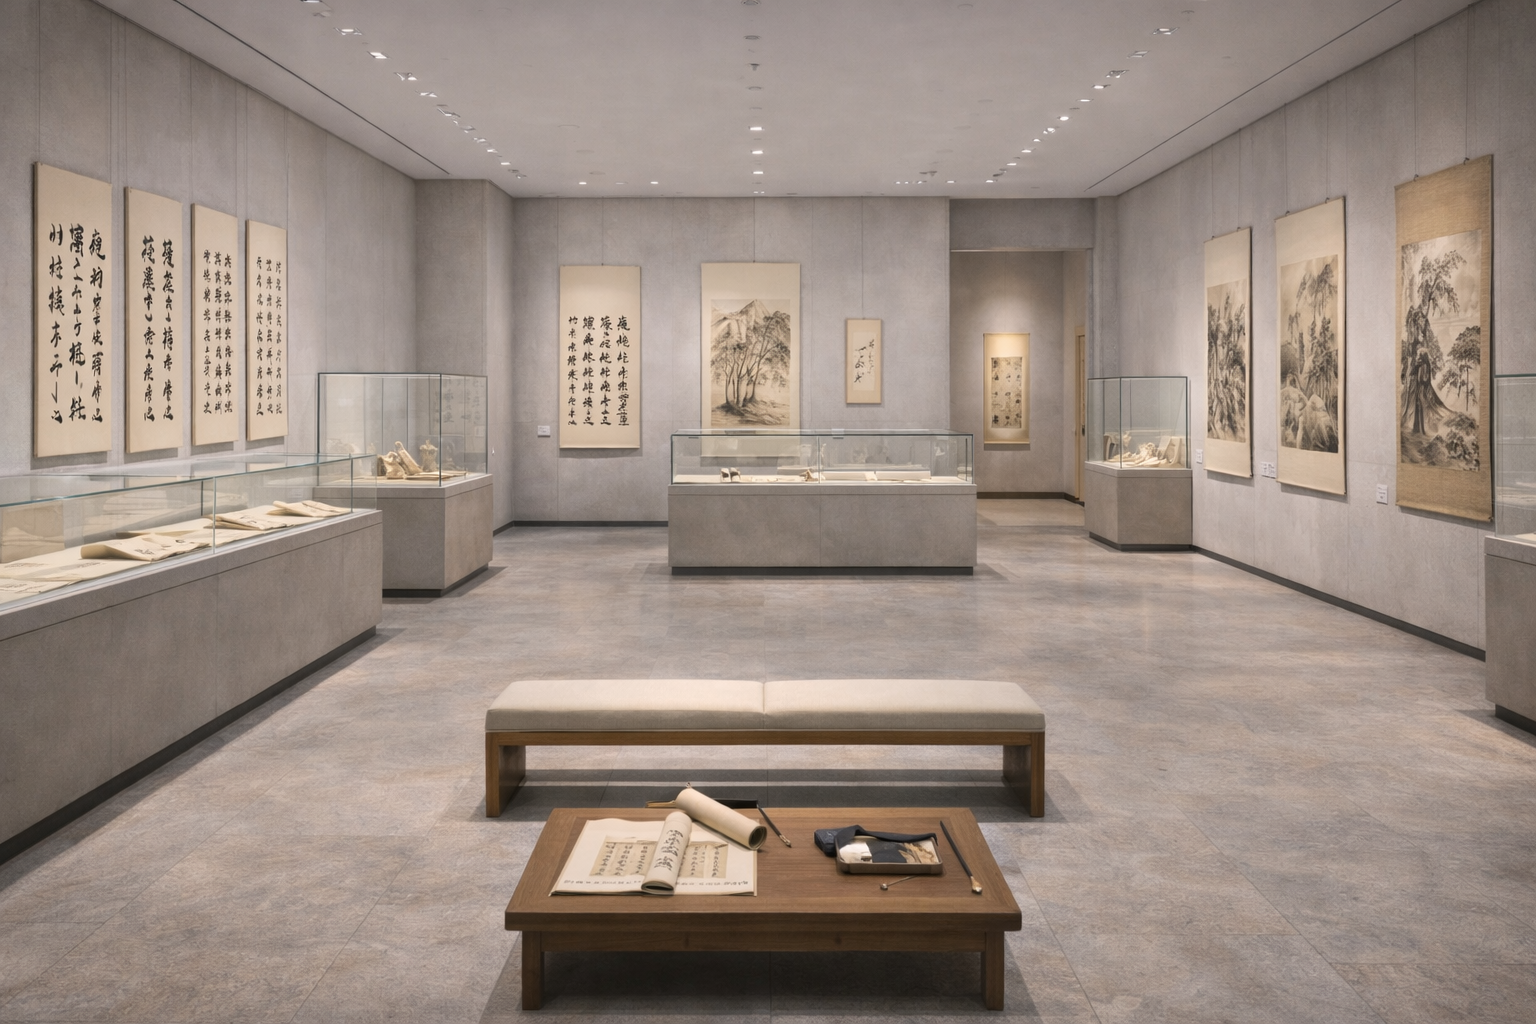
\includegraphics[width=\textwidth]{figure/figs/空间与展品设计.png}
    \captionof{figure}{空间与展品设计示意图}
    \label{fig-space-exhibit-design}
\end{center}

综上，空间及展品设计在本系统中承担着导览环境构建、路径组织、主题分段与对象承载的多重作用。通过展馆-楼层-展厅-展品的层级化空间组织、面向导览节奏的主题分区、强调代表性与可衔接性的展品配置，以及空间与展品的一体化联动设计，系统得以更自然地支持现场导览中的路径引导、对象聚焦与内容推进，使数字人导览在空间层和内容层上都更贴合真实参观体验。

\section{本章小结}
本章围绕面向博物馆导览的对话式数字人系统，完成了从目标定义到交互实现要素的整体设计说明。首先，在系统目标与整体架构层面，明确了系统以导览推进为核心任务，围绕观众在真实参观中的观看、提问、理解与跟随行为组织交互流程，并通过系统与 CCEG 三维能力的映射关系建立了从理论框架到设计实现的对应路径。随后，在对话组织设计中，本文从展品知识结构、分层讲解策略与探索式提问引导三个方面展开，形成了面向导览推进的内容组织机制，使讲解能够在概览、识别、深入与延展之间连续推进。

其次，在情境状态设计层面，本文分别构建了空间位置状态、导览对象状态、用户参观状态与导览进程状态，形成了面向现场导览的状态维护体系。该体系使系统能够持续判断“观众在哪里、正在看什么、处于何种参观阶段、导览已推进到哪里”，并据此完成讲解深度调节、对象切换、路径组织与转场决策。在具身交互设计层面，本文进一步从人物形象与性格、动作状态与注意力引导、语音风格与语调节奏、空间及展品环境四个维度完成实现性描述，使数字人的视觉形象、语言表达与导览任务保持一致。综合而言，本章将前文提出的框架要求落实为可执行的系统设计，为下一章开展实验与分析提供了完整的实现基础与评估对象。
